% ============================================================
% TA-IND-01 — Informe Académico Individual
% Análisis crítico de Apache Kafka frente a RabbitMQ
% Compilar: pdflatex -> biber -> pdflatex -> pdflatex
% ============================================================
\documentclass[12pt,a4paper]{article}

\usepackage[utf8]{inputenc}
\usepackage[T1]{fontenc}
\usepackage[spanish,es-tabla]{babel}
\usepackage{csquotes}
\usepackage[margin=2.5cm]{geometry}
\usepackage{graphicx}
\usepackage{float}
\usepackage{caption}
\usepackage{booktabs}
\usepackage{tabularx}
\usepackage{xcolor}
\usepackage{tikz}
\usepackage[hidelinks]{hyperref}
\usepackage[backend=biber,style=ieee]{biblatex}
\addbibresource{referencias.bib}

\graphicspath{{figuras/}{capturas/}{anexos/}}

% ---------- Datos de la carátula ----------
\newcommand{\estudiante}{Rivas Piloso Dayver Yahir}
\newcommand{\paralelo}{Séptimo nivel -- Paralelo B}
\newcommand{\fechaentrega}{15 de noviembre de 2026}
\newcommand{\repo}{https://github.com/drivasp/TA-IND-01-Kafka}

\begin{document}

% ============================================================
% 1. CARÁTULA
% ============================================================
\begin{titlepage}
  \centering
  \IfFileExists{figuras/logo_uteq.jpeg}{
\includegraphics[width=0.28\textwidth]{logo_uteq.jpeg}\par\vspace{0.8cm}}{}
  {\Large\bfseries UNIVERSIDAD TÉCNICA ESTATAL DE QUEVEDO\par}
  \vspace{0.4cm}
  {\large Facultad de Ciencias de la Computación\par}
  {\large Carrera de Software\par}
  \vspace{1cm}
  {\large\bfseries Aplicaciones Distribuidas (ISR-701)\par}
  \vspace{0.2cm}
  {\paralelo\par}
  \vspace{1cm}
  {\large\bfseries TA-IND-01 --- Informe Académico Individual\par}
  \vspace{0.2cm}
  {\large Análisis crítico de Apache Kafka frente a RabbitMQ\par}
  \vfill
  \begin{tabular}{rl}
    \textbf{Estudiante:} & \estudiante \\
    \textbf{Docente:}    & Gleiston Cicerón Guerrero Ulloa, PhD \\
    \textbf{Fecha:}      & \fechaentrega \\
    \textbf{Periodo:}    & SPA 2026-2027 \\
    \textbf{Repositorio:} & \url{\repo} \\
  \end{tabular}
  \vspace{1cm}
\end{titlepage}

% ============================================================
% 2. RESUMEN (150 a 200 palabras)
% ============================================================
\begin{abstract}
% Sistema analizado, enfoque y conclusiones principales.
\end{abstract}

\newpage
\tableofcontents
\newpage

% ============================================================
% 3. INTRODUCCIÓN
% ============================================================
\section{Introducción}
% Qué problema resuelve Kafka, quién lo usa, a qué escala y por qué se eligió.

% ============================================================
% 4. ARQUITECTURA DEL SISTEMA
% ============================================================
\section{Arquitectura del sistema}
% Componentes (brokers, tópicos, particiones, réplicas, productores,
% consumidores, controladores KRaft) y cómo se comunican.

\begin{figure}[H]
  \centering
  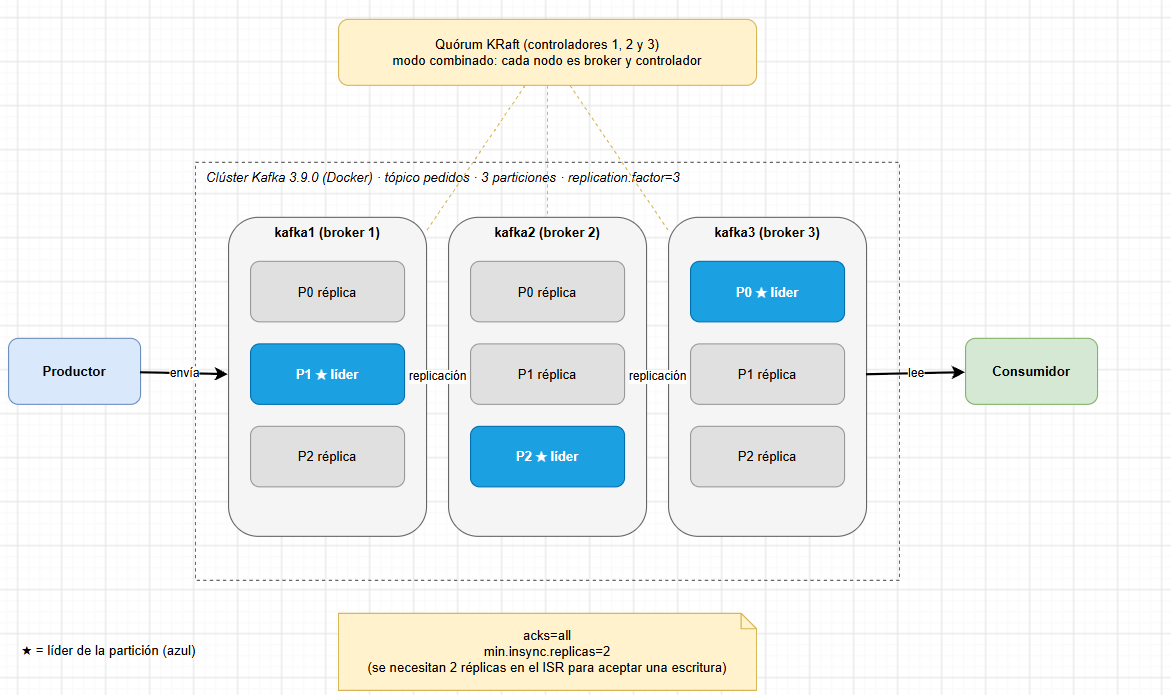
\includegraphics[width=0.95\textwidth]{arquitectura.png}
  \caption{Arquitectura del clúster Kafka usado en el experimento: tres brokers en modo KRaft, tópico \texttt{pedidos} con tres particiones y factor de replicación 3. El líder de cada partición se marca con una estrella ($\star$) (elaboración propia).}
  \label{fig:arquitectura}
\end{figure}
% Evolución desde el esquema a mano: ver Anexo~\ref{anexo:a}.

% ============================================================
% 5. ANÁLISIS CON LOS CONCEPTOS DE LA UNIDAD 1
% ============================================================
\section{Análisis con los conceptos de la Unidad 1}

\subsection{Transparencias de distribución}
% Acceso, ubicación, migración, reubicación, replicación, concurrencia y fallos.
% Cuáles ofrece y cuáles no, y por qué.

\subsection{Teorema CAP y PACELC}
% Qué prioriza con partición y qué prioriza sin partición. Con evidencia citada.

\subsection{Modelos de comunicación}
% Cliente-servidor, P2P o híbrido; síncrona o asíncrona; sockets, RPC o mensajería.

\subsection{Tolerancia a fallos}
% Qué fallos soporta, cómo los detecta y cómo se recupera. Incidente real documentado.

% ============================================================
% 6. EXPERIMENTACIÓN PROPIA
% ============================================================
\section{Experimentación propia}\label{sec:experimentacion}

\subsection{Entorno y configuración}
El experimento se montó en Windows con Docker Desktop v4.99.0 y la imagen oficial \texttt{apache/kafka:3.9.0}. Se configuró un clúster de tres nodos (\texttt{kafka1}, \texttt{kafka2} y \texttt{kafka3}) en modo KRaft, sin Apache ZooKeeper. Sobre ese clúster se creó el tópico \texttt{pedidos} con tres particiones y factor de replicación 3 (\texttt{replication.factor=3}). Se fijó un mínimo de 2 réplicas sincronizadas (\texttt{min.insync.replicas=2}) y el productor se configuró con confirmación total (\texttt{acks=all}). Con estos parámetros, cada escritura debe quedar confirmada en al menos dos réplicas antes de responder al cliente, así que la caída de un nodo no provoca pérdida de mensajes confirmados. Los comandos y archivos de configuración usados están en \texttt{experimento/comandos.md}.

\begin{figure}[H]
  \centering
  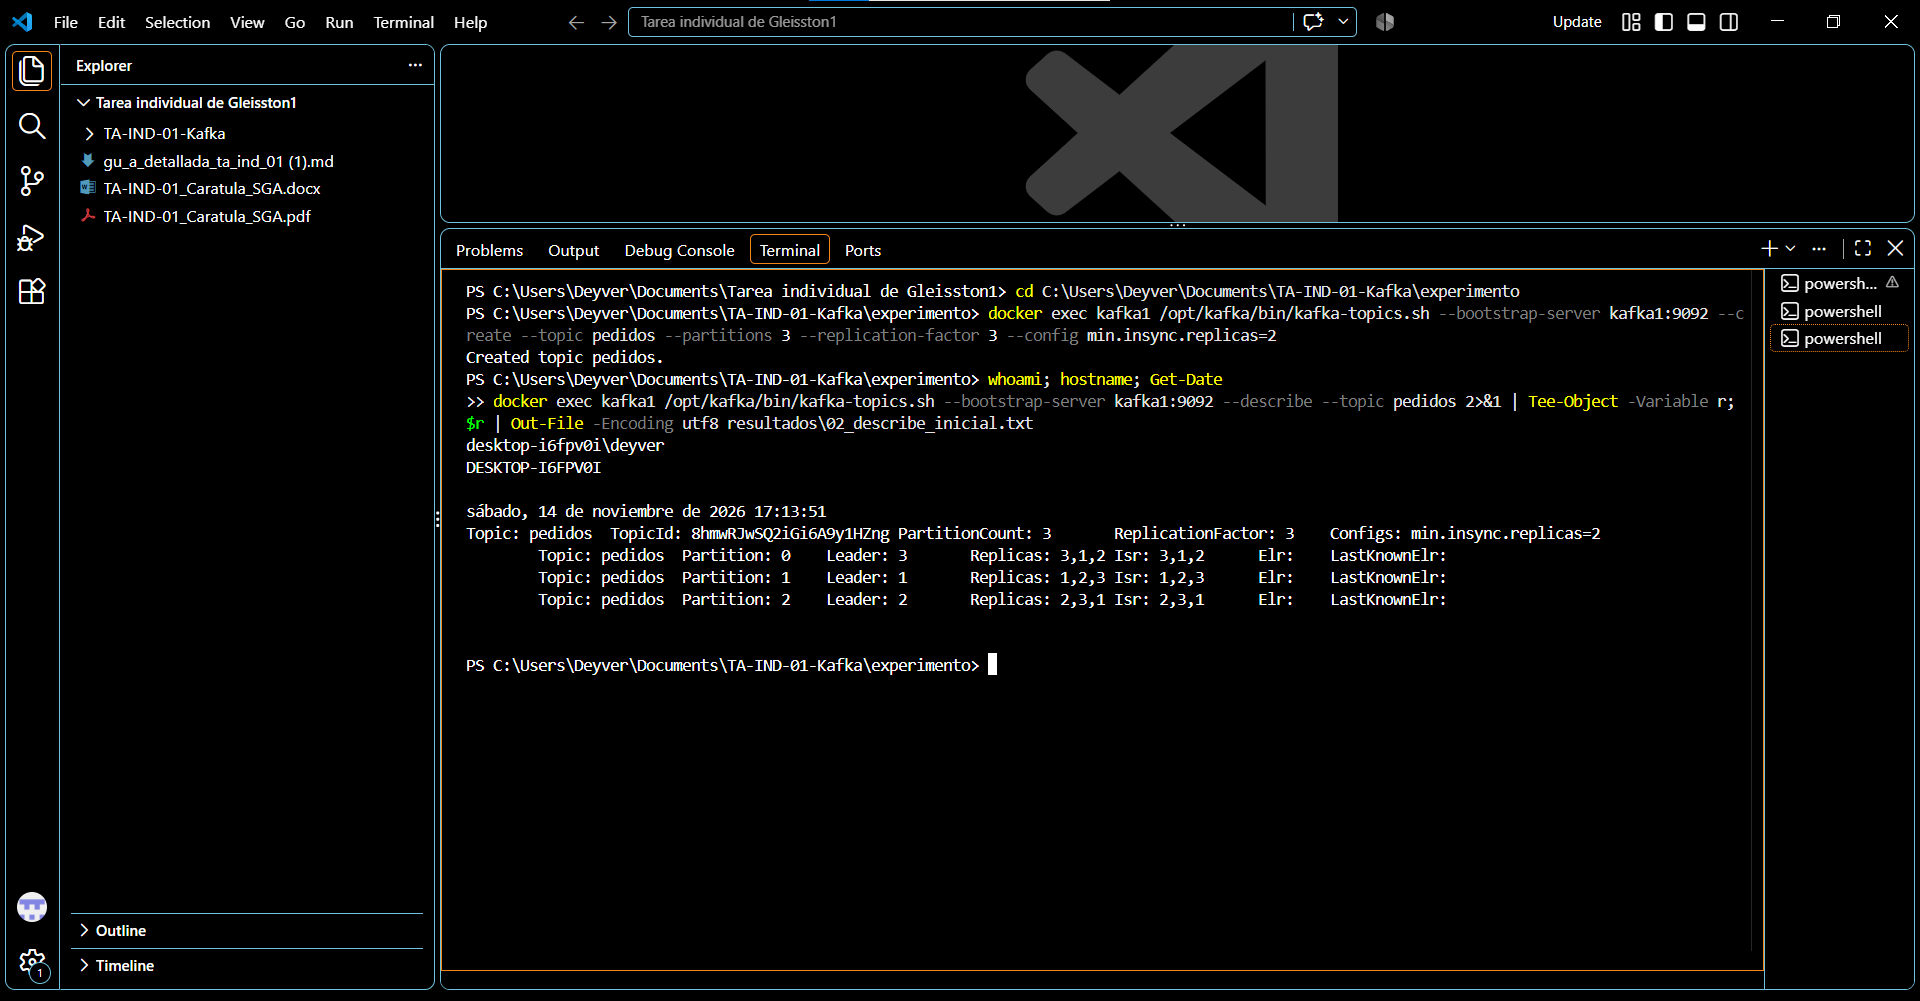
\includegraphics[width=0.95\textwidth]{sistema/capturaA_topico_estado_inicial.png}
  \caption{Estado inicial del tópico \texttt{pedidos}: distribución de liderazgo y conjunto ISR completo.}
  \label{fig:capA}
\end{figure}

\subsection{Prueba 1: caída del líder}
Para probar el comportamiento ante la caída de un nodo, se detuvo el contenedor \texttt{kafka3}, que era el líder de la partición 0 en el estado inicial (Figura~\ref{fig:capA}). Tras la desconexión, el controlador KRaft promovió al broker 1 (\texttt{kafka1}) como nuevo líder de esa partición, y el conjunto de réplicas sincronizadas (ISR) bajó de 3 a 2 nodos en todas las particiones. Luego se publicó el mensaje \texttt{pedido-4}: la escritura se aceptó y el consumidor recuperó los 4 mensajes acumulados sin pérdida de información (Figura~\ref{fig:capB}).

Con los conceptos de la Unidad 1, este resultado muestra tolerancia a fallos por replicación activa y reelección automática del líder~\cite{Raptis2023,Maharjan2023}. También muestra transparencia de ubicación y de fallos parcial: los clientes se conectaron a \texttt{kafka1} y siguieron operando sin intervención manual y sin saber qué broker tenía el liderazgo. La escritura de \texttt{pedido-4} no se bloqueó porque las 2 réplicas que quedaban en el ISR cumplían el mínimo de \texttt{min.insync.replicas=2}.

\begin{figure}[H]
  \centering
  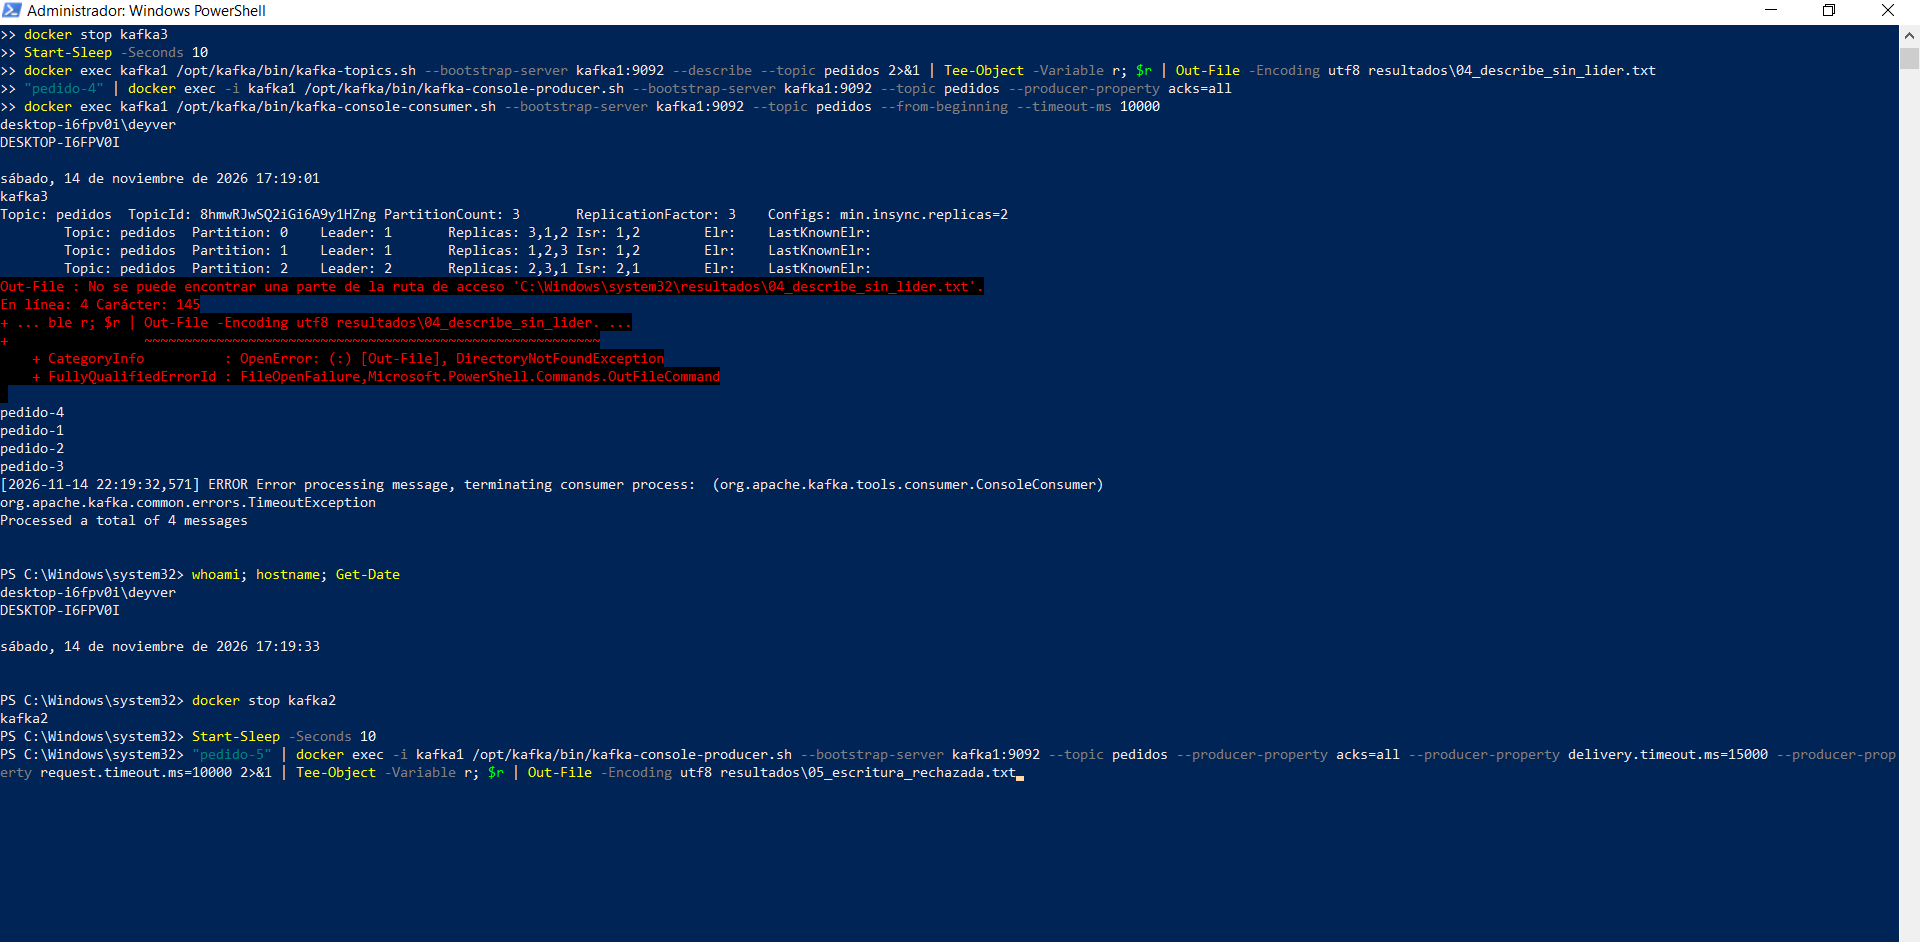
\includegraphics[width=0.95\textwidth]{sistema/capturaB_caida_lider_kafka3.png}
  \caption{Tras detener \texttt{kafka3}, el broker 1 asume el liderazgo de la partición 0 y el ISR se reduce a dos réplicas.}
  \label{fig:capB}
\end{figure}

\subsection{Prueba 2: pérdida del quórum de réplicas}
Después, con \texttt{kafka3} todavía detenido, se detuvo también \texttt{kafka2} y quedó activo solo \texttt{kafka1}. Al intentar enviar el mensaje \texttt{pedido-5}, el productor agotó sus reintentos tras recibir tres respuestas de error seguidas y rechazó la escritura con el error \texttt{NOT\_ENOUGH\_REPLICAS} (\texttt{NotEnoughReplicasException}), como se ve en la Figura~\ref{fig:capC}\footnote{Las marcas de tiempo de los registros muestran las 22:20 porque el contenedor usa horario UTC; equivale a las 17:20 en hora local de Ecuador (UTC$-5$).}.

El error indica que las réplicas sincronizadas bajaron del mínimo de 2 exigido por la configuración. Además, con solo 1 de 3 nodos activos se perdió la mayoría del quórum de votantes KRaft. En términos del teorema CAP, el sistema priorizó la consistencia (C) y la durabilidad de los mensajes confirmados por encima de la disponibilidad (A) en escritura: Kafka rechazó la petición en lugar de confirmar un dato guardado en una sola réplica, que se perdería si ese nodo fallara. Si \texttt{min.insync.replicas} estuviera en 1, el clúster habría aceptado \texttt{pedido-5} a favor de la disponibilidad, con el riesgo de perder el mensaje si \texttt{kafka1} fallaba antes de replicarlo~\cite{Wang2015}.

\begin{figure}[H]
  \centering
  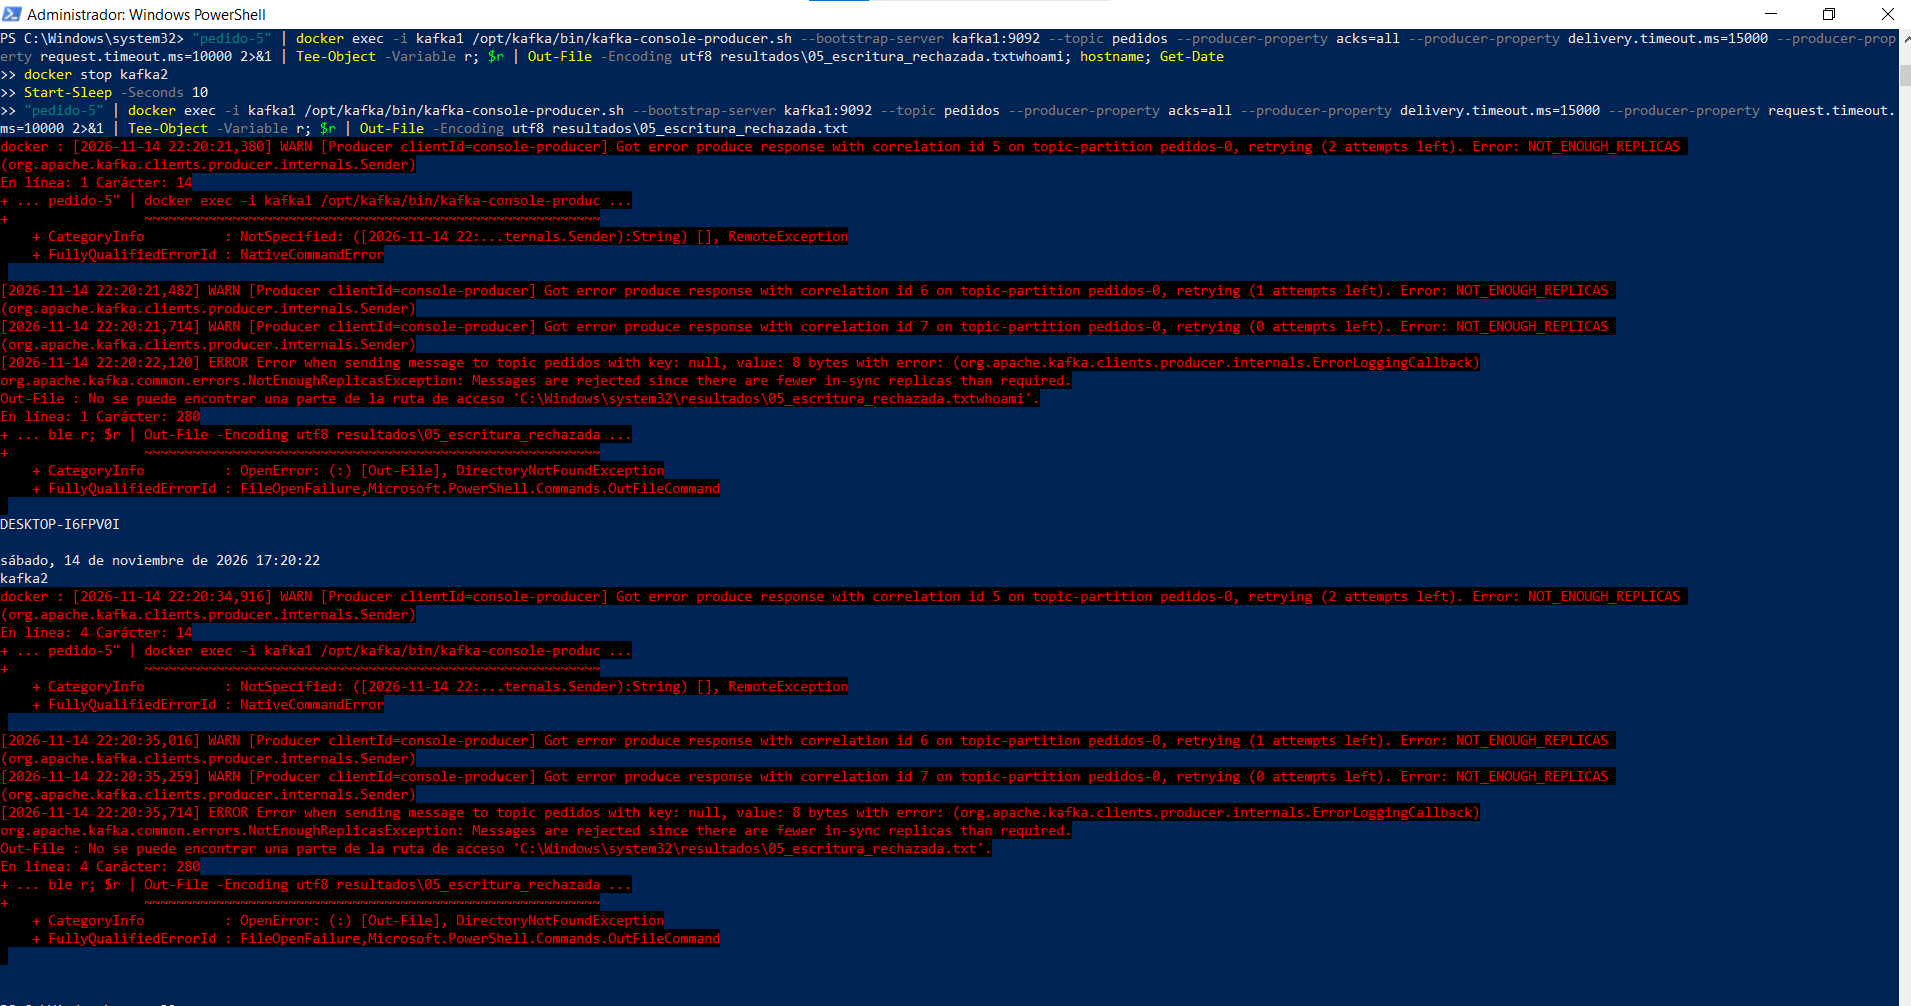
\includegraphics[width=0.95\textwidth]{sistema/capturaC_escritura_rechazada_not_enough_replicas.png}
  \caption{Con un solo broker activo, la escritura de \texttt{pedido-5} se rechaza con \texttt{NOT\_ENOUGH\_REPLICAS}.}
  \label{fig:capC}
\end{figure}

\subsection{Recuperación}
Por último, se reiniciaron los contenedores \texttt{kafka2} y \texttt{kafka3}. El clúster replicó los registros pendientes, el ISR volvió a tener 3 nodos en todas las particiones y el liderazgo de la partición 0 regresó a su líder preferido original (broker 3), como se ve en \texttt{experimento/resultados/06\_describe\_recuperado.txt}. El ciclo completo muestra el compromiso de diseño de esta configuración: para asegurar la durabilidad de los datos, Kafka bloquea las escrituras mientras los nodos activos estén por debajo del umbral definido.

% ============================================================
% 7. EJEMPLOS DEL ENTORNO DEL ESTUDIANTE
% ============================================================
\section{Ejemplos del entorno del estudiante}
% Al menos dos sistemas reales usados de primera mano, relacionados con un concepto.

% ============================================================
% 8. ANÁLISIS COMPARATIVO
% ============================================================
\section{Análisis comparativo}

\begin{table}[H]
  \centering
  \caption{Comparación entre Apache Kafka y RabbitMQ}
  \label{tab:comparacion}
  \begin{tabularx}{\textwidth}{@{}lXX@{}}
    \toprule
    \textbf{Criterio} & \textbf{Apache Kafka} & \textbf{RabbitMQ} \\
    \midrule
    Transparencias &  &  \\
    CAP (con partición) &  &  \\
    PACELC (sin partición) &  &  \\
    Modelo de comunicación &  &  \\
    Replicación &  &  \\
    Detección y recuperación de fallos &  &  \\
    \bottomrule
  \end{tabularx}
\end{table}

% Discusión de la tabla.

% ============================================================
% 9. POSTURA CRÍTICA
% ============================================================
\section{Postura crítica}
% Fortalezas, limitaciones, trade-offs y contextos en los que no sería la mejor opción.

% ============================================================
% 10. CONCLUSIONES
% ============================================================
\section{Conclusiones}

% ============================================================
% 11. DECLARACIÓN DE USO DE IA
% ============================================================
\section{Declaración de herramientas utilizadas}

Para el desarrollo técnico, la gestión bibliográfica y la maquetación del presente informe se emplearon las siguientes herramientas de apoyo, manteniendo la autoría intelectual y el análisis crítico a cargo del estudiante:

\begin{itemize}
  \item \textbf{Claude (Anthropic, modelo Claude Opus 5.5, noviembre de 2026):} Utilizado como asistente técnico para estructurar el código fuente en LaTeX, reescribir la redacción de la Sección~\ref{sec:experimentacion} a partir de un borrador basado en mis apuntes experimentales, localizar fuentes bibliográficas recientes (\cite{Raptis2023,Raptis2024,Maharjan2023,Kaczor2022,Wang2022KRaft}) y formatear sus metadatos en \texttt{referencias.bib}.
  \item \textbf{Docker Desktop (v4.99.0) y Apache Kafka (v3.9.0):} Empleados para el despliegue local del clúster de tres nodos en modo KRaft y la ejecución controlada de las pruebas de tolerancia a fallos y teorema CAP.
  \item \textbf{draw.io (diagrams.net):} Utilizado por el estudiante para diseñar y elaborar manualmente el diagrama arquitectónico de la Figura~\ref{fig:arquitectura}, a partir de los datos de su propio experimento.
  \item \textbf{TeX Live / Biber:} Utilizados para la compilación del documento fuente (\texttt{main.tex}) y la generación automatizada de referencias en formato IEEE.
\end{itemize}

\textbf{Autoría y método de verificación:} El diseño del experimento, el levantamiento de los contenedores, la ejecución de comandos, la captura de evidencias y el diseño y elaboración manual del diagrama arquitectónico de la Figura~\ref{fig:arquitectura} en draw.io (diagrams.net) fueron realizados por el autor. Toda sugerencia de redacción, formato o referencia generada por la IA fue verificada manualmente: se contrastaron los valores técnicos de la Sección~\ref{sec:experimentacion} contra las salidas crudas (\texttt{06\_describe\_recuperado.txt}) y las Figuras~\ref{fig:capA}--\ref{fig:capC}, y se validó cada DOI directamente en Crossref y en los portales de las revistas para confirmar la exactitud de autores, volúmenes y páginas.

% ============================================================
% 12. REFERENCIAS (IEEE, biblatex)
% ============================================================
\printbibliography[heading=bibintoc,title={Referencias}]

% ============================================================
% 13. ANEXOS
% ============================================================
\appendix
\renewcommand{\thesection}{\Alph{section}}

\section{Esquema inicial a mano}\label{anexo:a}
\begin{figure}[H]
  \centering
  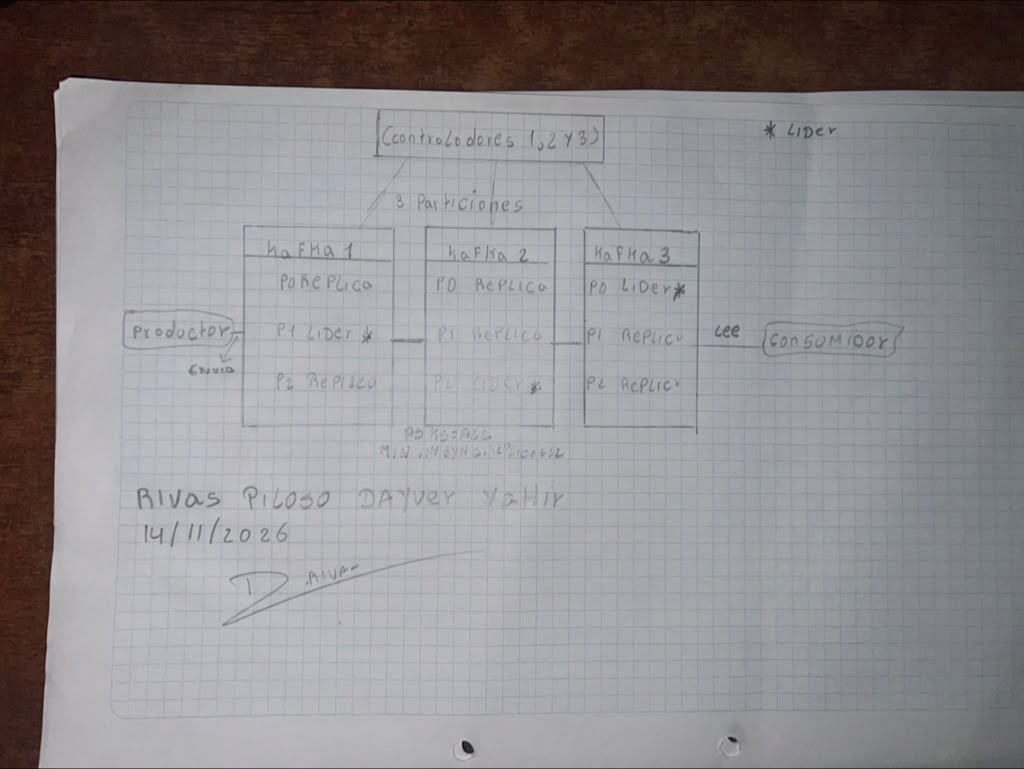
\includegraphics[width=0.9\textwidth]{esquema_mano.jpg}
  \caption{Esquema inicial a mano del clúster: productor, tres brokers con sus particiones P0, P1 y P2 (líder y réplicas), controladores KRaft y consumidor.}
  \label{fig:esquema_mano}
\end{figure}

\section{Capturas de lectura de las fuentes}\label{anexo:b}

\begin{figure}[H]
  \centering
  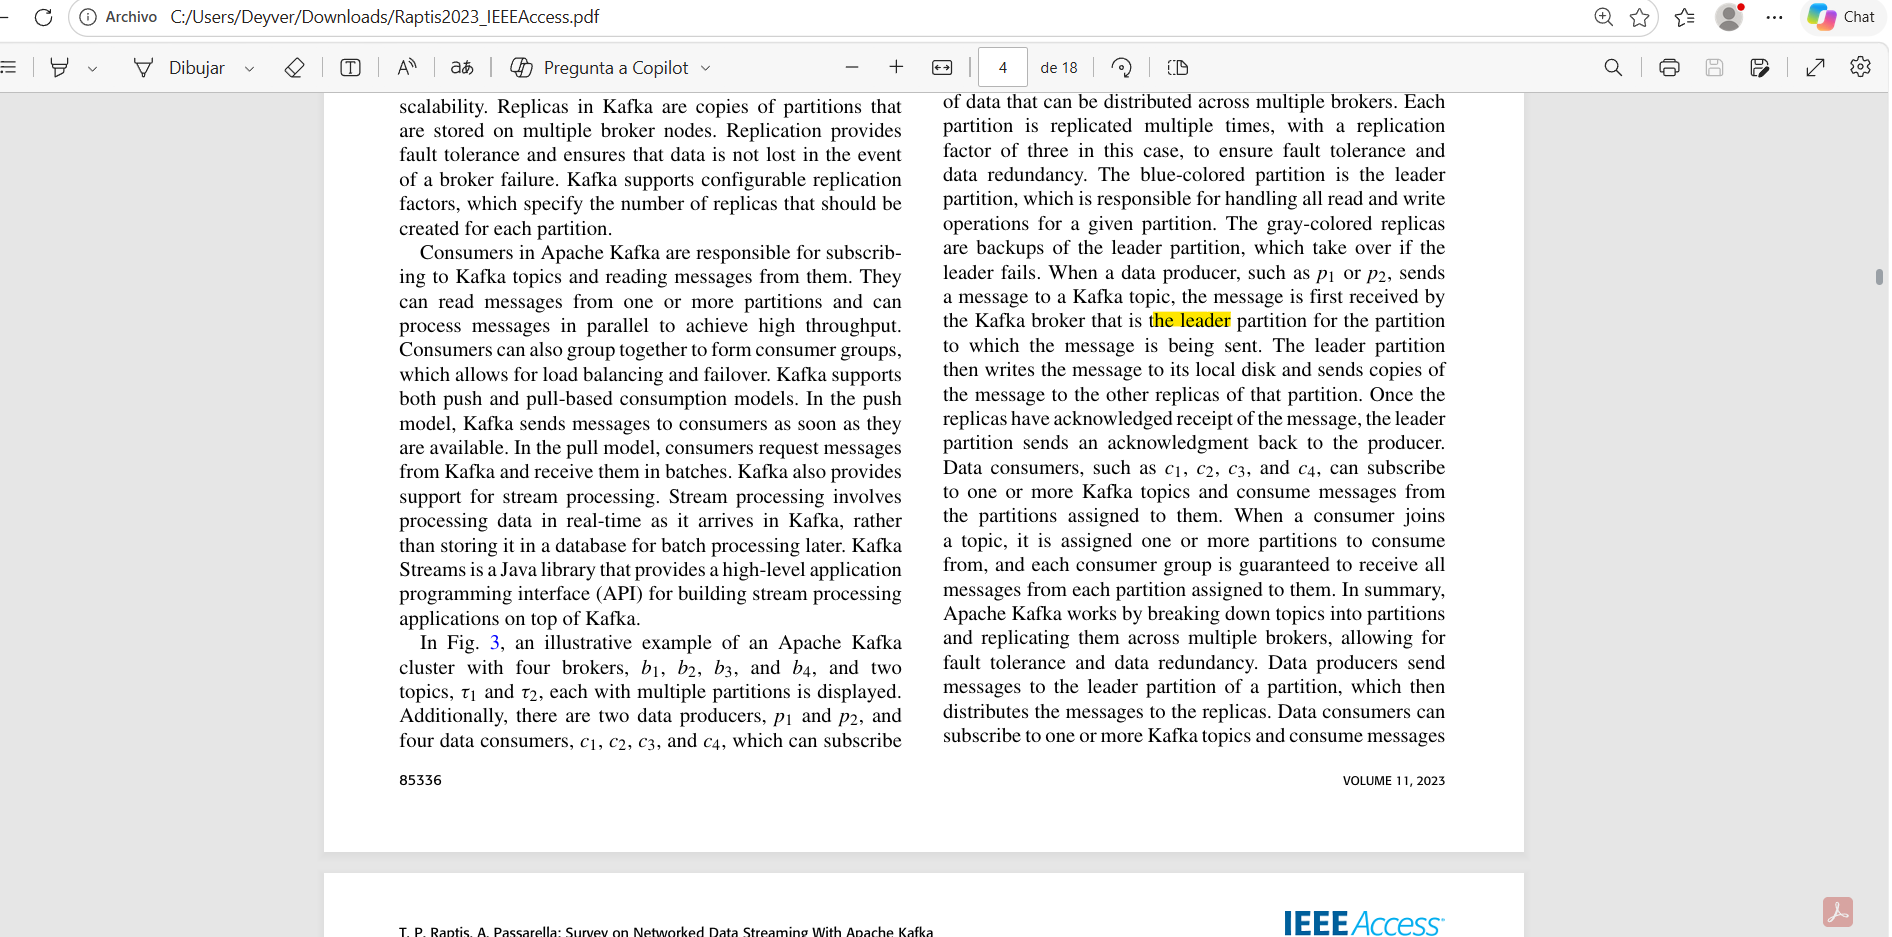
\includegraphics[width=0.95\textwidth]{fuentes/fuente1_raptis.png}
  \caption{Raptis y Passarella~\cite{Raptis2023}, p.~85336. Cada partición tiene un líder que atiende lecturas y escrituras, y las réplicas lo reemplazan si falla. Se usa en la Prueba~1 (Sección~\ref{sec:experimentacion}).}
  \label{fig:fuente1}
\end{figure}

\begin{figure}[H]
  \centering
  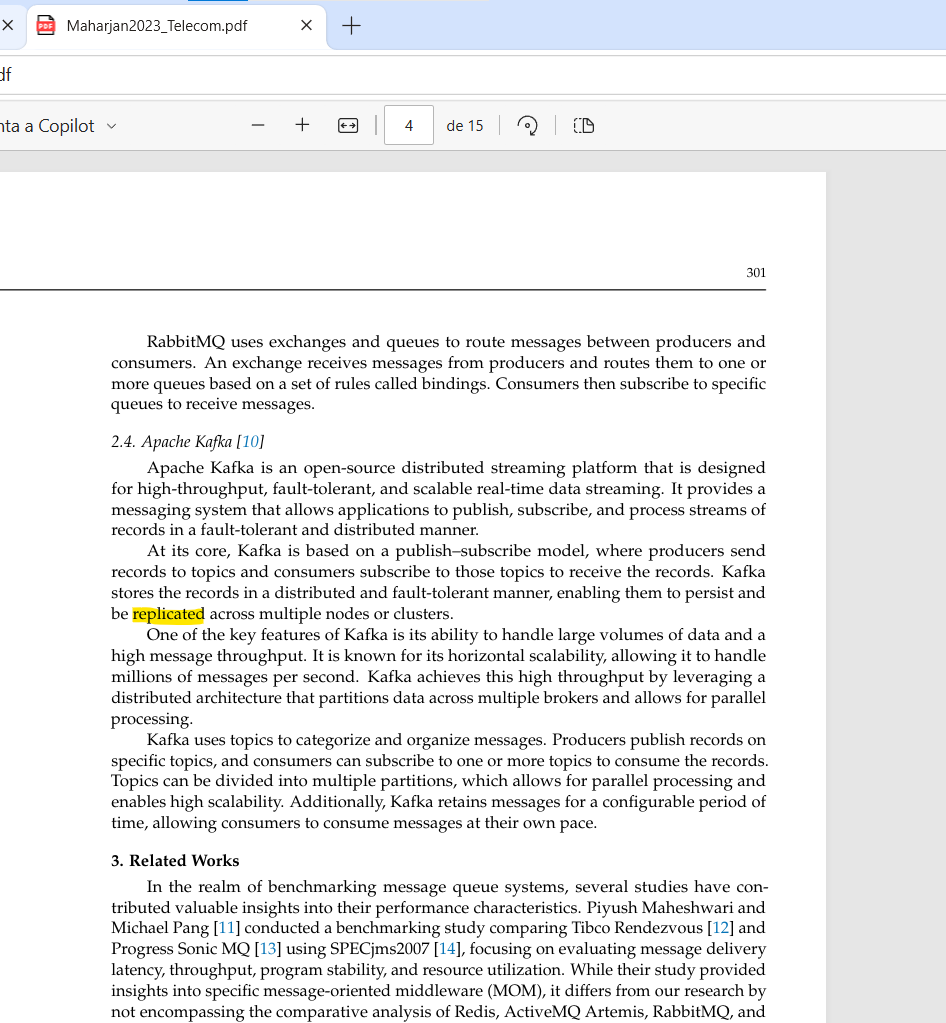
\includegraphics[width=0.6\textwidth]{fuentes/fuente2_maharjan.png}
  \caption{Maharjan et al.~\cite{Maharjan2023}, p.~301. Kafka guarda los registros de forma distribuida y tolerante a fallos, replicados en varios nodos. Se usa en la Prueba~1 (Sección~\ref{sec:experimentacion}).}
  \label{fig:fuente2}
\end{figure}

\begin{figure}[H]
  \centering
  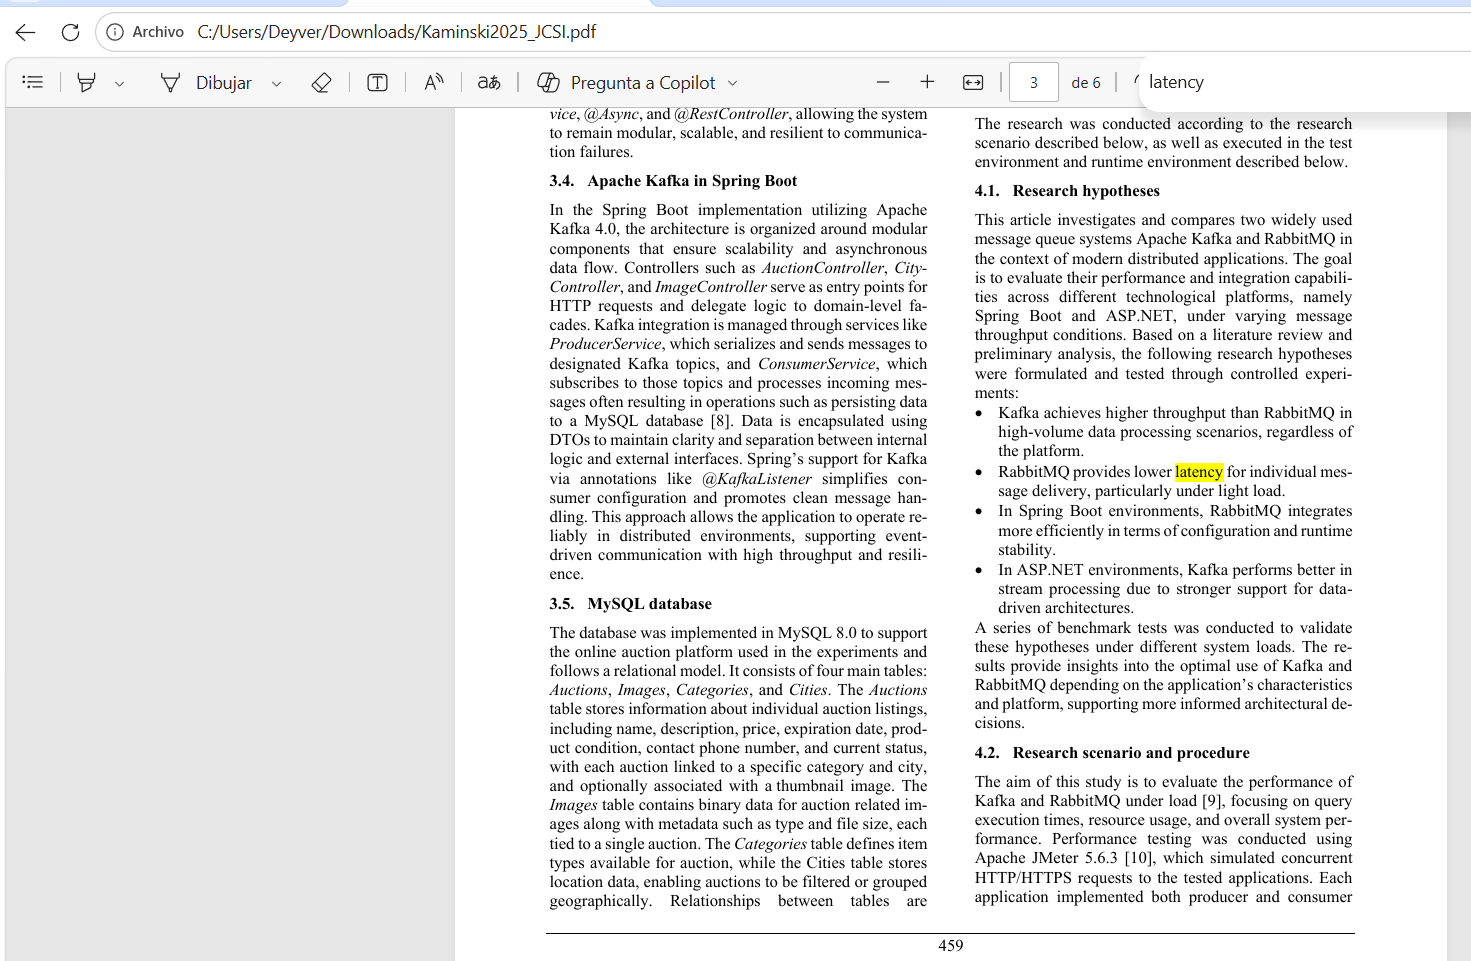
\includegraphics[width=0.95\textwidth]{fuentes/fuente3_kaminski.png}
  \caption{Kamiński et al.~\cite{Kaminski2025}, p.~459. Hipótesis del estudio: RabbitMQ ofrece menor latencia en la entrega de mensajes individuales, sobre todo con poca carga.}
  \label{fig:fuente3}
\end{figure}

\end{document}
